% I only need the arrows for this one.
%\usepackage{tikz}
%\usetikzlibrary{arrows}
% Place the TikZ picture in a figure environment.
%\begin{figure}
%\centerline{
  % Resize it to 5cm wide.
%\resizebox{horizontal length}{vertical length}{material}
  \resizebox{.3\linewidth}{!}{
    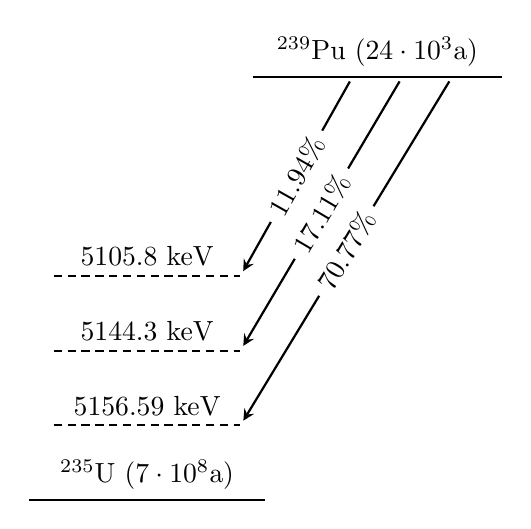
\begin{tikzpicture}[
      scale=0.45,
      level/.style={thick},
      virtual/.style={thick,densely dashed},
      trans/.style={thick,->,shorten >=2pt,shorten <=2pt,>=stealth},
      classical/.style={thin,double,<->,shorten >=4pt,shorten <=4pt,>=stealth}
    ]
    % Draw the energy levels.
    \draw[level] (20em,18em)    -- (40em,18em) node[midway,above] {$^{239}$Pu ($24\cdot10^3$a)};
    \draw[level] (2em,-16em)  -- (21em,-16em) node[midway,above] {$^{235}$U ($7\cdot10^8$a)};
    % Draw the virtual levels.
    \draw[virtual] (4em, 2em)  -- (19em, 2em)  node[midway,above] {5105.8 keV};
    \draw[virtual] (4em,-4em)  -- (19em, -4em)  node[midway,above] {5144.3 keV};
    \draw[virtual] (4em,-10em) -- (19em, -10em) node[midway,above] {5156.59 keV};
    % Draw the transitions.
    \draw[trans] (28em, 18em) -- node[sloped,fill=white] {$11.94\%$} (19em, 2em);
    \draw[trans] (32em, 18em) -- node[sloped,fill=white] {$17.11\%$} (19em, -4em);
    \draw[trans] (36em,18em) -- node[sloped,fill=white] {$70.77\%$} (19em,-10em);
    %    \draw[classical] (4.5cm,-8em) -- (1.5cm,-5em) node[midway,below] {\Ga{}};
    \end{tikzpicture}
  }
%}
%\caption{Zerfallschema}
%\end{figure}


%  \begin{comment}
%  http://www.nndc.bnl.gov/nudat2/decaysearchdirect.jsp?nuc=Pu239&unc=nds
%  
%  Author: E. BROWNE   Citation:Nuclear Data Sheets 98, 665 (2003)
%  
%  Half-Life: 24110 a
%  
%  Alphas:
%  
%  Energy (keV)	Intensity (%)	Dose ( MeV/Bq-s )
%  ...
%  ...
%    4529.6	     3.19E-6 % 3 	  1.445E-7 14 
%    4534	     2.84E-6 % 5 	  1.288E-7 23 
%    4559	     1.2E-5 % 5 	  5.5E-7 23 
%    4632 3 	     7.0E-4 % 20 	  3.2E-5 9 
%    4655	     2.8E-6 % 6 	  1.3E-7 3 
%    4691 3 	     5.0E-4 % 20 	  2.3E-5 9 
%    4718.5	     4.00E-5 % 10 	  1.89E-6 5 
%    4736 3 	     0.0051 % 8 	  2.4E-4 4 
%    4749 5 	     6.0E-4 % 6 	  2.8E-5 3 
%    4769 5 	     0.0015 % 6 	  7E-5 3 
%    4795 4 	     0.0012 % 6 	  6E-5 3 
%    4824	     2.30E-5 % 20 	  1.11E-6 10 
%    4828 3 	     0.0024 % 7 	  1.2E-4 3 
%    4866 5  ?	     0.0019 % 7 	  9E-5 3 
%    4871 5 	     7E-4 % 3 	  3.4E-5 15 
%    4912 5 	     0.0024 % 9 	  1.2E-4 4 
%    4934 3 	     0.0060 % 10 	  3.0E-4 5 
%    4960 5 	     0.0070 % 10 	  3.5E-4 5 
%    4987 3 	     0.0130 % 20 	  6.5E-4 10 
%    5006 5 	     0.0170 % 20 	  8.5E-4 10 
%    5028 3 	     0.009 % 3 	  4.5E-4 15 
%    5054 5 	     0.047 % 13 	  0.0024 7 
%    5076 5 	     0.078 % 8 	  0.0040 4 
%  *  5105.5 8 	    11.94 % 7 	  0.610 4 
%    5111 ?	     0.010 % 10 	  5E-4 5 
%  *  5144.3 8 	    17.11 % 14 	  0.880 7 
%  *  5156.59 14 	    70.77 % 14 	  3.649 7 
%    5156.7	     0.030 % 3 	  0.00155 15 
%  \end{comment}
